% pdf/a 
\begin{filecontents*}[overwrite]{\jobname.xmpdata}
    \Title{Önálló laboratórium 2 dolgozat}
    \Author{Szilágyi Gábor}
    \Language{hu-HU}
    \Subject{Modell-redukció alkalmazása az elektromágneses térszámításban}
    \Keywords{POD}
    \Publisher{Szilágyi Gábor}
\end{filecontents*}

\documentclass[a4paper,12pt,titlepage]{article}
\usepackage{ucs}
\usepackage[T1]{fontenc}
\usepackage[utf8]{inputenc}
\usepackage[magyar]{babel}
\usepackage{amsfonts}
\usepackage{amsmath,bm}
%\usepackage{amssymb}
\usepackage{graphicx}
%\usepackage[hang]{caption}
%\usepackage{subcaption}
%\usepackage{enumerate}
%\usepackage{psfrag}
\usepackage{siunitx}
\usepackage[left=20mm,right=20mm,top=20mm,bottom=25mm]{geometry}
%\usepackage[left=10mm,right=10mm,top=10mm,bottom=15mm]{geometry} %landscape
%\usepackage[hyphenbreaks]{breakurl}
%\usepackage[hyphens]{url}
%\usepackage{multirow}
%\usepackage{booktabs}
\usepackage{hyperref}
%\usepackage{listings}
%\usepackage{cite}
%\usepackage{csquotes}
%\usepackage[range-phrase=--, range-units=single]{siunitx}
\usepackage{xcolor}
\usepackage[a-3u]{pdfx}
\hypersetup{
    colorlinks,
%    linkcolor={red!50!black},
    linkcolor={black},
%    citecolor={blue!50!black},
    citecolor={black},
%    urlcolor={blue!80!black}
    urlcolor={blue!80!black}
}

\sloppy % Margón túllógó sorok tiltása.
\widowpenalty=10000 \clubpenalty=10000 %A fattyú- és árvasorok elkerülése
\def\hyph{-\penalty0\hskip0pt\relax} % Kötőjeles szavak elválasztásának engedélyezése

\pagestyle{plain} 

\listfiles % a package-ek kilistázása a logba

\title{
    \centering
    
\includegraphics[width=0.6\textwidth]{kep/bme_logo.pdf} \\
    \vspace{0.5cm}
    \large{\bf Budapesti Műszaki és Gazdaságtudományi Egyetem \\
    Villamosmérnöki és Informatikai Kar \\
    Szélessávú Hírközlés és Villamosságtan Tanszék}\\
    \vspace{4cm}
    \large{Önálló laboratórium 2 dolgozat} \\
    \vspace{2cm}
    \Large{\bf{Modell-redukció alkalmazása az elektromágneses térszámításban}} \\
    \vspace{2cm}
}

%\parskip=10pt
%\parindent=0pt

\newcommand\adj[1]{#1^{\mathrm{H}}}

\author{Szilágyi Gábor \\\vspace{2cm}\\ Konzulens: Dr. Bilicz Sándor}
\date{Budapest, \today}


\begin{document}
    \maketitle
    \setcounter{page}{2}
    \tableofcontents
    \section{Bevezetés}
            A POD, vagyis a Proper Orthogonal Decomposition, egy bázistranszformációs eljárás, ami egy adott adathalmaz reprezentálásához optimális bázist keres meg. Az eljárás által meghatározott $\Psi$ bázisban a bázisvektoroknak az a tulajdonsága, hogy a lehető legkevesebb bázisvektorral leírható az adathalmaz információtartalmának vagy energiájának lehető legnagyobb része. Ezt felhasználva a $\Psi$ csonkításával egy $\Psi'$ közelítő bázist lehet előállítani, ami lényegesen kisebb rendű, mint $\Psi$, mégis kis hibával reprezentálható benne az eredeti adathalmaz. Természetesen minél több bázisvektort hagyunk meg $\Psi'$-ben, annál jobban csökken a modell-redukcióból származó hiba, de a csonkítás mértékét az adott alkalmazáshoz mérten előírhatjuk. A POD egy másik előnyös tulajdonsága, hogy a gyakorlati esetek nagy részében a sorbarendezett $\psi_n$ bázisvektorokra eső energiatartalom rohamosan csökken, ezért sokszor nagyságrendekkel kisebb dimenziószámú bázissal is jól leírható az adathalmaz, mint az eredeti esetben.
        \subsection{A módszer eredete}
            A módszer gyökerei az '40-es évekig nyúlnak vissza, amikor olyan tudományos problémákat próbáltak statisztikai módszerekkel megközelíteni, amelyeknek a megoldása valamilyen folytonos értékű függvény, sok esetben sztochasztikus folyamat. Egy jeles személy ebből a kezdeti időszakból Damodar Dharmananda Kosambi \cite{Kosambi11} indiai matematikus, aki a POD alapját képező (Kosambi--)Karhunen–Lo\`eve Expansion, vagyis Karhunen–Lo\`eve felbontás atyja. A Karhunen–Lo\`eve felbontás sztochasztikus folyamatok olyan reprezentálását teszi lehetővé, ahol a sztochasztikus folyamatot egy végtelen összeg alakjában írjuk fel. Ha ebből az összegből csak az első véges sok $n$ db. tényezőt hagyjuk meg (csonkítjuk a felbontást), akkor a kapott összegnek a lehető legkisebb a négyzetes hibája az eredeti sztochasztikus folyamathoz képest \cite{Aadithya18}.
            \par
            
        \subsection{Felhasználási területekről általában}
            Az eljárást számos tudományterületen sikeresen alkalmazták már, különböző területeken különböző néven szokták emlegetni gyakorlatilag ugyanezt az eljárást. Statisztikában főként Principal Component Analysis (PCA) néven fordul elő és nagy adathalmazok információtartalmának kinyerésére használják \cite{Jolliffe16}. Ahogy fent emlytettem, találkozhatunk még vele az irodalomban Karhunen–Lo\`eve Expansion néven is, elsősorban a sztochasztikus folyamatok kapcsán \cite{Aadithya18}. A turbulens áramlások kutatásával kapcsolatban pedig Method of Snapshots néven is ismert az 1980-as évektől \cite{Sirovich}.
            \par
            Lényeges felhasználási területek például: turbulens áramlások szimulációja; statisztikában és más területeken az adathalmazok redukálása \cite{Jolliffe16}; szabályozástechnikában a szuboptimális, de gyorsan számítható beavatkozás; nemlineáris elektromágneses problémák (pl. motorok) szimulációja \cite{Henneron14}.
        \subsection{Problémakörök}
            A felsorolt problémák, amelyeknél segítséget nyújthat a POD, különböző kategóriákba sorolhatóak.
            \par
            Elsősorban statisztikában merül fel az a gond manapság, hogy egy nagyon sok bejegyzést tartalmazó adathalmaz áll rendelkezésre, amelynek minden bejegyzése sokdimenziós, emiatt az adatok által hordozott információ nehezen hasznosítható. Ez az információkinyerés annak ellenére is problémás, hogy a sok rendelkezésre álló adat összesen sok információt hordoz magában. Ekkor a POD (PCA) segítségével kinyerhetők az adathalmazt jól leíró, jellegzetes mintázatok, amelyek a hasznos információ nagy részét magukban hordozzák.
            \par
            A szimulációk esetében más a helyzet. Itt az jelenti a gondot, hogy a szimulált modell nagyon részletes, például nagyon sok (könnyen $10^6$ -- $10^9$ nagyságrendű) végeselemet tartalmaz, emiatt a szimuláció futtatása sok számítógép erőforrást használ fel. Egyrészt a megoldás memóriában való tárolása is problémás lehet, másrészt a végeselemek módszerénél maradva nagyon nagy egyenletrendszert kell megoldani, ami sok processzoridőt igényel, ami miatt sokáig tart a szimuláció. Ekkor a POD segítségével a ténylegesen megoldandó egyenletrendszer és a megoldás méretét is nagyságrendekkel csökkenteni lehet. Ez úgy történhet, hogy valamilyen előzetes szimuláció eredményét felhasználva az adott modellhez tartozó jellegzetes részmegoldások lineáris kombinációjaként igyekszünk előállítani egy az eredeti modellhez képest is közelítő megoldást, aminek sokkal kisebb az erőforrásigénye.
        \subsection{Alkalmazás az elektromágneses térszámításban}
            \label{sec:empod}
            Az EM térszámításban többféle kontextusban is hasznos lehet a POD a futási idő  vagy a memóriafelhasználás jelentős csökkentésére. Az egyik megközelítésben egy időtartománybeli végeselem modellben zajló tranziens folyamat lefolyására kaphatunk számítás szempontjából olcsó, közelítő megoldást. Ehhez először a teljes kérdéses időintervallum első töredék részére egy teljes értékű szimulációt futtatunk, amely viszonylag sok számítást igényel. Ennek a rövid részmegoldásnak az eredményei szolgálnak a POD bemenetéüli. A POD ezek alapján meghatározza a rendszer dinamikájában megjelenő struktúrákat, majd csak a lényeges összetevőkre szorítkozva egy lecsökkentett szabadsági fokú rendszert szimulálunk tovább a hátralévő időben, ami már időlépésenként sokkal kevesebb számítást igényel.
            \par
            A fent vázolt, tranziens szimulációban történő alkalmazáson kívül más módokon is hasznosítható lehet a POD a térszámítási problémákban, de a dolgozatomban elsősorban ezzel a megközelítéssel foglalkozom.
            %TODO
    \section{A POD-ról részletesebben}
        A bevezetésben említettem, hogy az adathalmaz energiájának vagy információtartalmának szempontjából optimális a $\Psi$ bázis, de ez pontosításra szorul.
        %TODO pontosítás
        \subsection{A felbontás egyenletei}
            A redukálandó adathalmaz méreteitől függően különböző számítási módok optimálisak a POD redukált bázisának előállításához. Az eredeti adathalmazt egy mátrixba rendezzük úgy, hogy az egyes mintákhoz artozó adatok vektorai (${\bf x}_i \in \mathbb{C}^n,~i \in \{1,~\hdots,~k\}$) a mátrix oszlopvektorai legyenek. Az így kapott mátrix (${\bf S}$) a snapshotmátrix vagy mintamátrix:
            \begin{align}
                {\bf S} = & \left[ {\bf x}_1~{\bf x}_2~{\bf x}_3~\hdots~{\bf x}_k \right]
            \end{align}
            Az adott alkalmazástól függ, hogy ${\bf S}$-nek melyik mérete olyan nagy, hogy az gondot jelentsen. \Aref{sec:empod}. részben vázolt nagy szabadsági fokú szimulációknál az okozza a gondot, hogy az egy időlépéshez tartozó ${\bf x}_i$ dimenziószáma -- vagyis $n$ -- nagy, könnyen milliós nagyságrendű, miközben egy jó redukált bázis előállításához, $k \ll n$ db. ${\bf x}_i$ minta elég a dinamikus rendszerből. Ebben az esetben jól használható az ${\bf S}$ szinguláris érték szerinti felbontása (Singular Value Decomposition, SVD):
            \begin{align}
                \label{equ:svd}
                {\bf S}~=&~{\bf U \Sigma \adj{V}}
            \end{align}
        \subsection{Az egyenletek értelmezése}
            Itt érdemes megállni és értelmezni a felbontásban szereplő mátrixokat és azok jelentését a modellezett rendszerrel kapcsolatban. \Aref{equ:svd}. egyenletben ${\bf U} \in \mathbb{C}^{n\times k}$ lesz a teljes $\Psi$ bázis vektorait (${\bf u}_i,~i \in \{1,~\hdots,~k\}$), mint oszlopvektorokat tartalmazó unitér mátrix, tehát az oszlopai egységvektorok. A ${\bf \Sigma} \in \mathbb{R}^{m\times m}~(m=min\{n,k\}=k)$ egy pozitív definit diagonálmátrix, aminek az $i$-eik diagonálelemei, $\sigma_i$ az ${\bf u}_i$-hez tartozó együttható, ami azt fejezi ki, hogy az adott bázisvektor mennyire fontos, mennyire járul hozzá általában a rendszer állapotához, más szóval a rendszer energiájának vagy információtartalmának mekkora része írható le az adott bázisvektorral. A ${\bf \Sigma}$ olyan felépítésű az SVD miatt, hogy a diagonálelemek csökkenő sorrendben szerepelnek az átlóban bal fentről jobbra lefelé haladva. A ${\bf U\Sigma} \in \mathbb{C}^{n\times m}$ szorzat tehát már az eredeti adatokhoz skálázott bázisvektorok mátrixának tekinthető, amelyben fontosság szerint csökkenő sorrendben szerepelnek egymás után a bázisvektorok. Tömören összefoglalva a ${\bf \adj{V}}$ mátrix a skálázott bázisvektorokhoz tartozó együtthatók mátrixa. A ${\bf \adj{V}}$ mátrix az $i$-edik ${\bf v}_i$ oszlopában tartalmazza az ${\bf x}_i$ mintavektor előállításához szükséges együtthatókat, amelyek a ${\bf U\Sigma}$ szorzat oszlopait súlyozzák:
            \begin{align}
                {\bf x}_i~=&~{\bf U\Sigma v}_i
            \end{align}
            Más szemszögből megközelítve a ${\bf \adj{V}}$ értelmezését, $v_{j,i}$, tehát ${\bf \adj{V}}$ $j$-edik sorának $i$-edik eleme (${\bf v}_i$ $j$-edik eleme) jelenti ${\bf u}_j \sigma_j$ hozzájárulását vagy súlyát ${\bf x}_i$-hez.
            \par
            Az ellenkező esetben, amikor $k$ nagy és emiatt $m=min\{n,k\}=n$, már számításigény szempontjából nem optimális ${\bf S}$ teljes SVD-jének direkt kiszámolása, mert ez az immár $k \times k$ méretű ${\bf \adj{V}}$ mátrix kiszámolásával jár, ami a redukált modell létrehozása szempontjából lényegtelen. Ebben az esetben érdemesebb kiszámítani az adathalmaz kovarianciamátrixát, a ${\bf C} \in \mathbb{C}^{n \times n}$ mátrixot. Azért jutunk ezzel előrébb, mert \aref{equ:kovariancia}. egyenletben látható módon az ${\bf U}$ mátrixot megkaphatjuk a ${\bf C}$ spektrálfelbontásából is. Mivel ${\bf C}$ szimmetrikus, ezért pozitív definit, emiatt mindig létezik spektrálfelbontása.
            \begin{align}
            \begin{split}
                \label{equ:kovariancia}
                {\bf C}~=&~{\bf S \adj{S}} \\
                =&~{\bf U \Sigma \adj{V} V\Sigma \adj{U}} \\
                =&~{\bf U \Sigma}^2{\bf \adj{U}}
            \end{split}
            \end{align}
            Itt ${\bf S}$ a snapshot-mátrix, ${\bf U}$ oszlopai az új bázisvektorok, ${\bf \Sigma}$ tartalmazza a bázisvektorok információtartalmát jellemző szinguláris értékeket a főátlójában, ${\bf \adj{V}}$ sorai az egyes bázisvektorok időfüggő együtthatói, ${\bf C}$ pedig az ${\bf x}_i$ mintavektorokból álló adathalmaz kovarianciamátrixa.
        \subsection{Az SVD takarékos változatai}
            Az SVD algoritmusnak többféle változata ismert, amelyek mind műveletszám, mind memóriahasználat terén takarékosabbak a teljes SVD-nél. Ahogy már fent is említettem, a redukált bázis meghatározása szempontjából a ${\bf V}$ mátrix kiszámolása érdektelen.
            %TODO wikipedia szerint thin, compact és truncated. Lehet, hogy föntebb is át kéne írni, hogy hogy érdemes kiszámolni 
    \section{Példa szimuláció}
        A POD működésének demonstrálására a konzulensem, Dr. Bilicz Sándor segítségével írtam egy MATLAB szkriptet. A szkript egy egydimenziós véges differencia közelítést használó modell tranziens viselkedését szimulálja, pontosabban az elektromos és mágneses tár alakulását. A megoldást többféleképpen számítja ki, teljes és redukált bázisú változatban is, hogy ezek összehasonlíthatóak legyenek.
        \subsection{A modell}
            A szimulációval egy kör keresztmetszetű, $a$ sugarú, végtelen hosszú, véges vezetőképességű vezetőben létrejövő mágneses és elektromos teret vizsgáltam. \Aref{fig:modell}. ábrán látható módon áll össze a modell. 
            \par
            \begin{figure}[h]
                \centering
                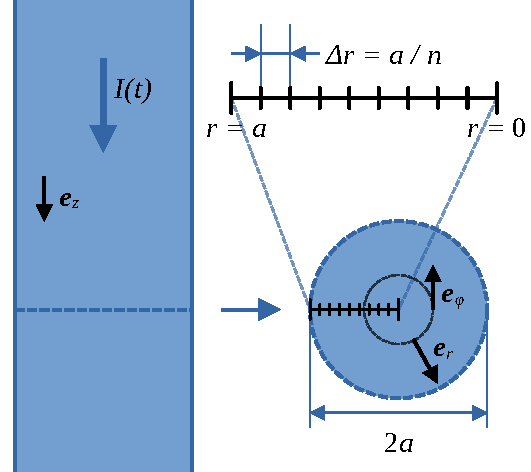
\includegraphics[width=0.5\textwidth]{kep/modell.pdf}
                \caption{A szimulált modell}
                \label{fig:modell}
            \end{figure}
             A vezető rúd keresztmetszete a szaggatottal jelölt kör. A használt hengerkoordinátarendszer bázisvektorai ${\bf e}_{z}, {\bf e}_{\phi}$ és ${\bf e}_{r}$. A vezető henger szimmetriatengelye $z$-irányú és szintén $z$-irányú benne a felületi áramsűrűség vektora is, ez az áramsűrűség a vezető hossza mentén nem változik. A modell általában $z$-irányú eltolásra és a szimmetriatengely körüli ($\varphi$ irányú) forgatásra invariáns, emiatt csak az egyes mennyiségek $r$ sugártól való függését kell vizsgálni, emiatt egydimenziós a modell.
             \par
             A vezető keresztmetszetére elő van írva az összesített áram időfüggvénye, $I(t)$, de a skin-hatás miatt a vezető belsejében nem egyenletes az áramsűrűség, hanem a sugár mentén haladva változik. Ugyanígy a vezető belsejében létrejövő $H_\varphi$ és $E_z$ is függ a sugártól. Ezek a mennyiségek továbbá időfüggőek is, de a vezető henger önindukciója miatt nem pontosan a gerjesztéssel együtt változnak. Ezeknek a mennyiségeknek az időbeli alakulása a kérdés, ezeket határozza meg a szimuláció egy adott gerjesztés mellett.
            \par
            A modell például egy villámhárító földelő vezetőjében létrejövő elektromágneses tér alakulásának a vizsgálatára használható, amikor a villám meghatározza a villámhárítón folyó áramot.
        \subsection{A számítás menete}
            A szimuláció
    \section{\LaTeX~Próba}
        Lorem ipsum \cite{PGD}.
        \begin{align}
            {\bf X}~=&~{\bf V\Sigma U}^*
        \end{align}
    \bibliography{mybib}
    \bibliographystyle{plain}
\end{document}

%\cite{Henneron14}

%            \begin{figure}
%                \centering
%                \includegraphics[width=0.8\textwidth]{kep/szerkesztett/wstk-mighty-gecko-nagy.jpg}
%                \caption{WSTK + radio board.}
%                \label{fig:wstkmighty}
%            \end{figure}
% \cite{Anritsu}
%            \begin{figure}
%                \centering
%                \begin{subfigure}{0.48\textwidth}
%                    \includegraphics[width=\textwidth]{kep/szerkesztett/sol-868-conducted.png}
%                    \caption{\SI{868}{MHz}}
%                \end{subfigure}
%                \begin{subfigure}{0.48\textwidth}
%                    \includegraphics[width=\textwidth]{kep/szerkesztett/sol-470-conducted.png}
%                    \caption{\SI{470}{MHz}}
%                \end{subfigure}
%                \caption{470 és \SI{868}{MHz}-es Sol radio board-ok kimeneti spektruma.}
%                \label{fig:sol-conducted}
%            \end{figure}

